%!TeX root=../tese.tex
%(dica para o editor de texto: este arquivo é parte de um documento maior)
% para saber mais: https://tex.stackexchange.com/q/78101/183146

\chapter{Redes neurais artificiais}
\label{cap:redes}

Neste capítulo são apresentados alguns conceitos básicos de \defi{aprendizado de máquina}, com foco nos algoritmos de redes neurais artificiais, em especial o \defi{perceptron}, cujo desenvolvimento foi inspirado nas redes neurais biológicas, ou seja, os neurônios e suas conexões no cérebro, conforme descrito por Kopec \citep{classic}.

Pode-se classificar as técnicas de aprendizado de várias formas, de acordo com alguma de suas características. Por exemplo, Géron \citep{hands} utiliza o grau de supervisão humana durante o seu funcionamento para classificá-los em aprendizado supervisionado ou não-supervisionado.

\section{Aprendizado de máquina supervisionado}

 Um algoritmo de \defi{aprendizado supervisionado} é usado quando conhecemos os rótulos dos dados que estamos utilizando para o treinamento, ou seja, temos a resposta correta da aprendizagem. Por exemplo, se estamos classificando fotos de animais, possuímos um conjunto de fotos em que já sabemos de antemão quais são de gatos, cachorros, etc.

 O ato de rotular ou classificar os dados que usamos no aprendizado é o que designamos de supervisão humana. Uma vez \emph{treinado}, o algoritmo recebe uma foto nova e então a classifica como sendo uma foto de um gato, ou cachorro, ou qualquer outra resposta daquelas que foram dadas como exemplos durante o treinamento.

Dentro do aprendizado supervisionado temos duas técnicas principais. A regressão é usada para prever valores, e a classificação é usada para prever os rótulos dos dados, que também são chamados de classes. Neste texto os termos ``algoritmo'' e ``técnica'' serão usados livremente como sinônimos, pois uma técnica de aprendizado de máquina, no contexto atual, é obviamente um algoritmo executado no computador.

Colocar exemplos...

\section{Aprendizado não-supervisionado}

Nesse tipo de aprendizado de máquina, não sabemos os rótulos dos dados que estamos lidando, assim o algoritmo poderá agrupar os dados de forma automática, por exemplo, se estiver sendo usado um algoritmo classificador.

Alguns métodos não-supervisionadas de aprendizado foram enumeradas por Géron \citep{hands}. O \textbf{agrupamento} de dados similares, sendo essa similaridade podendo ser uma distância no espaço dos dados (inspiração geométrica), e utiliza-se algoritmos como $k$-Vizinhos, $k$-Means, $k$-Medians, etc. Exemplos de aplicações são agrupamento de produtos em supermercados, interesses comuns de clientes em sites de conteúdo digital, etc.

Outra técnida é a \textbf{detecção de anomalias}, cujo objetivo é ter uma descrição de como os dados considerados ``normais'' se parecem, e usa esse agrupamento para detectar se novos dados estariam ``fora'' desse padrão. Um exemplo é a detecção de fraudes.

Também pode-se citar sobre a técnica de \textbf{estimação de densidades}, que tem como objetivo a estimação da função densidade de probabilidade de um conjunto de dados gerados por algum processo aleatório.

Colocar exemplos...

\section{Técnicas de classificação}

Sendo uma das duas técnicas principais do aprendizado supervisionado, problemas desse tipo buscam aprender com um conjunto de dados previamente rotulados, como ``se parecem'' os dados que pertencem às classes que queremos classificar, para que quando processarmos novos dados, o algoritmo usado possa identificar, o mais corretamente possível, as classes às quais pertecem esses dados, dentro do conjunto de classes que já definimos ao rotular os dados iniciais.

Existem vários tipos de algoritmos de classificação, dentre eles podemos mencionar: Máquina de Vetor Suporte, em inglês Support Vector Machine (SVM), Árvores de decisão, Florestas aleatórias (podendo ser entendidas como um conjunto de centenas de árvores de decisão aleatoriamente definidas) e as Redes neurais artificiais.

Colocar exemplos de aplicações...

Todos essas técnicas podem ser usadas para classificação linear ou não-linear, no sentido em que valores eles estão classificando, assim como na forma que está sendo feita essa classificação. Se imaginamos um espaço bidimensional, um algoritmo de classificação linear irá separar as classes de dados por retas, enquanto que um classificador não-linear poderá usar outra curva qualquer para a separação. Abstraindo o espaço bidimensional para os espaços multidimensionais dos dados que são comumente analisados, podemos pensar em hiperplanos (estruturas ($n{-}1$-dimensionais de espaços $n$-dimensionais) para o caso dos classificadores lineares, ou subespaços quaisquer para os não-lineares.

\section{Redes neurais}

Uma rede neural artificial é um dentre vários métodos de classificação, ou seja, de aprendizado supervisionado. De acordo com Kopec \citep{classic}, ele é utilizado como um classificador não-linear, e por isso pode ser utilizado para prever tipos de dados genéricos, que podem ou não ser lineares.

Kopec \citep{classic} também cita que apesar das primeiras redes neurais artificiais, ou \eng{perceptrons} tivessem sido desenvolvidas ainda na década de 1950, sob a inspiração do funcionamento do cérebro, nota-se que, de tempos pra cá, vem recebendo muita importância graças à evolução computacional de hardware e software desde o início dos anos 2000.

Contextualizar mais as redes neurais aqui ...

\section{Perceptron}

A rede neural mais simples, isto é, a primeira que foi criada, chama-se \eng{perceptron}. Mais recentemente surgiu a rede perceptron de várias camadas (\eng{multi-layer perceptron}), àquela mais simples e antiga dá-se o nome de perceptron de única camada (\eng{single-layer perceptron}), uma ilustração dela está na Figura ~\ref{fig:perceptron}. 

\begin{figure}[htb]
\centering
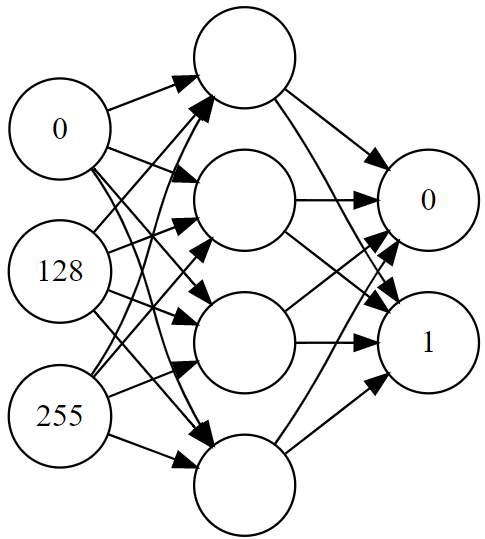
\includegraphics[width=6cm]{figuras/perceptron}
\caption{\label{fig:perceptron}Rede neural simples, o perceptron de única camada. }
\end{figure}

O perceptron de camada única consiste de uma camada de neurônios de entrada, uma camada oculta de neurônios usados na otimização, e uma camada de saída, que irá conter os dados previstos, ou ainda as probabilidades do dado pertencer a alguma das classes que a rede poderá classificá-lo.

Os neurônios são representados por círculos, cada coluna de neurônios representa uma camada, nesse caso, da esquerda para a direita temos a camada de entrada, a camada oculta e a camada de saída. As linhas representam as ligações entre os neurônios, sendo que cada neurônio de uma camada está ligado a todos da camada anterior.

Vou descrever aqui as contas...

\section{Sistemas nebulosos}

Os sistemas nebulosos foram criados a partir da teoria dos conjuntos nebulosos criada por \cite{fuzzy_1}

A partir disto, conforme descrito por \citep{fuzzy_2}, os sistemas nebulosos são aproximadores universais. Isto significa que podem aproximar quaisquer funções numa grande variedade de de problemas. Ainda neste artigo é descrito como uma função de 